\subsection{Data Normalization and Binning}

To reduce the number of classes to calculate the Naive Bayes for, then the data set is reduced by grouping the data into bins.
This can be done on various ways:

\begin{enumerate}
\item The pixel values can be grouped into 'x' number of groups.
This reduces the probability calculations to be done in the Naive Bayes. \label{list:bin}
\item Nearby pixels can be grouped together, which is the same as reducing the resolution.
\item PCA can be applied on the z-score normalized data to find the most significant variation in it and step \ref{list:bin} can then be applied. \label{list:pca_bin}
\end{enumerate}

From these methods, method \ref{list:pca_bin} was chosen.

Figure \ref{fig:effect_of_binning} shows the effect on a picture when the numbers are only binned.
The PCA and normalization can here, for good reasons, not be shown.


\begin{figure}[H]
\centering
    \begin{subfigure}{0.22\textwidth}
        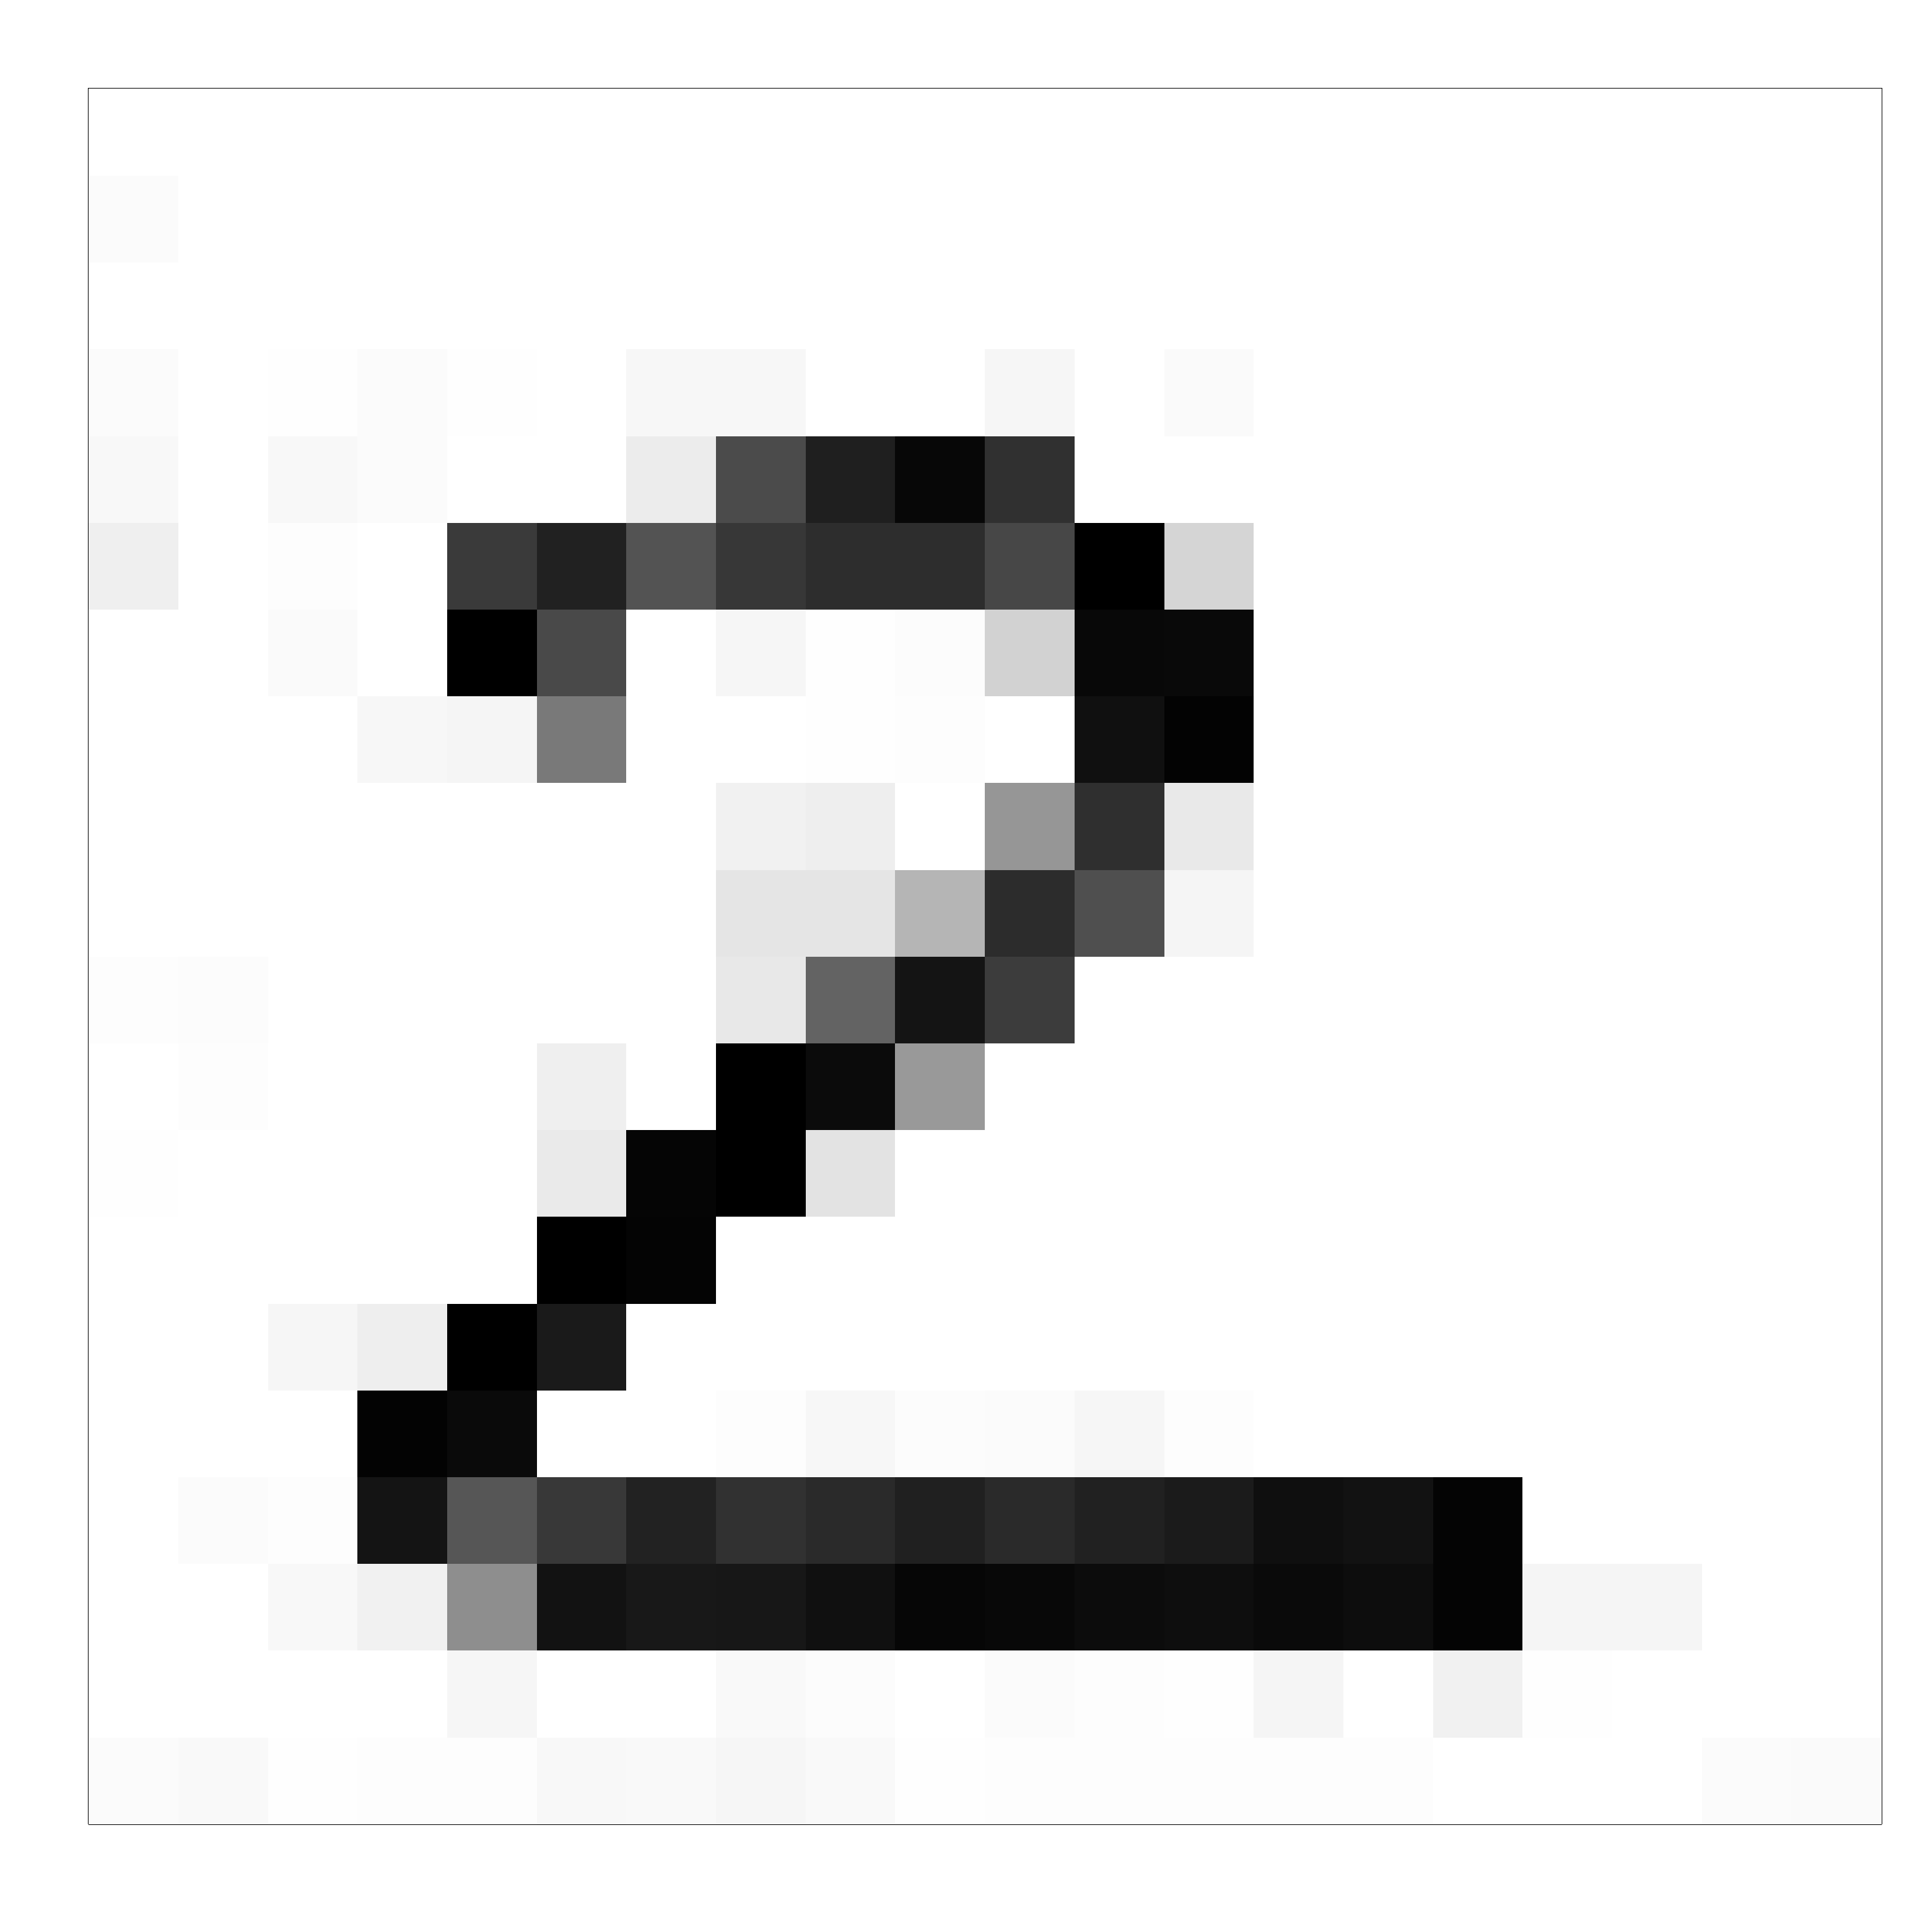
\includegraphics[width = \textwidth]{graphics/bins_inf}
        \caption{Raw image.}
    \end{subfigure}
    \begin{subfigure}{0.22\textwidth}
        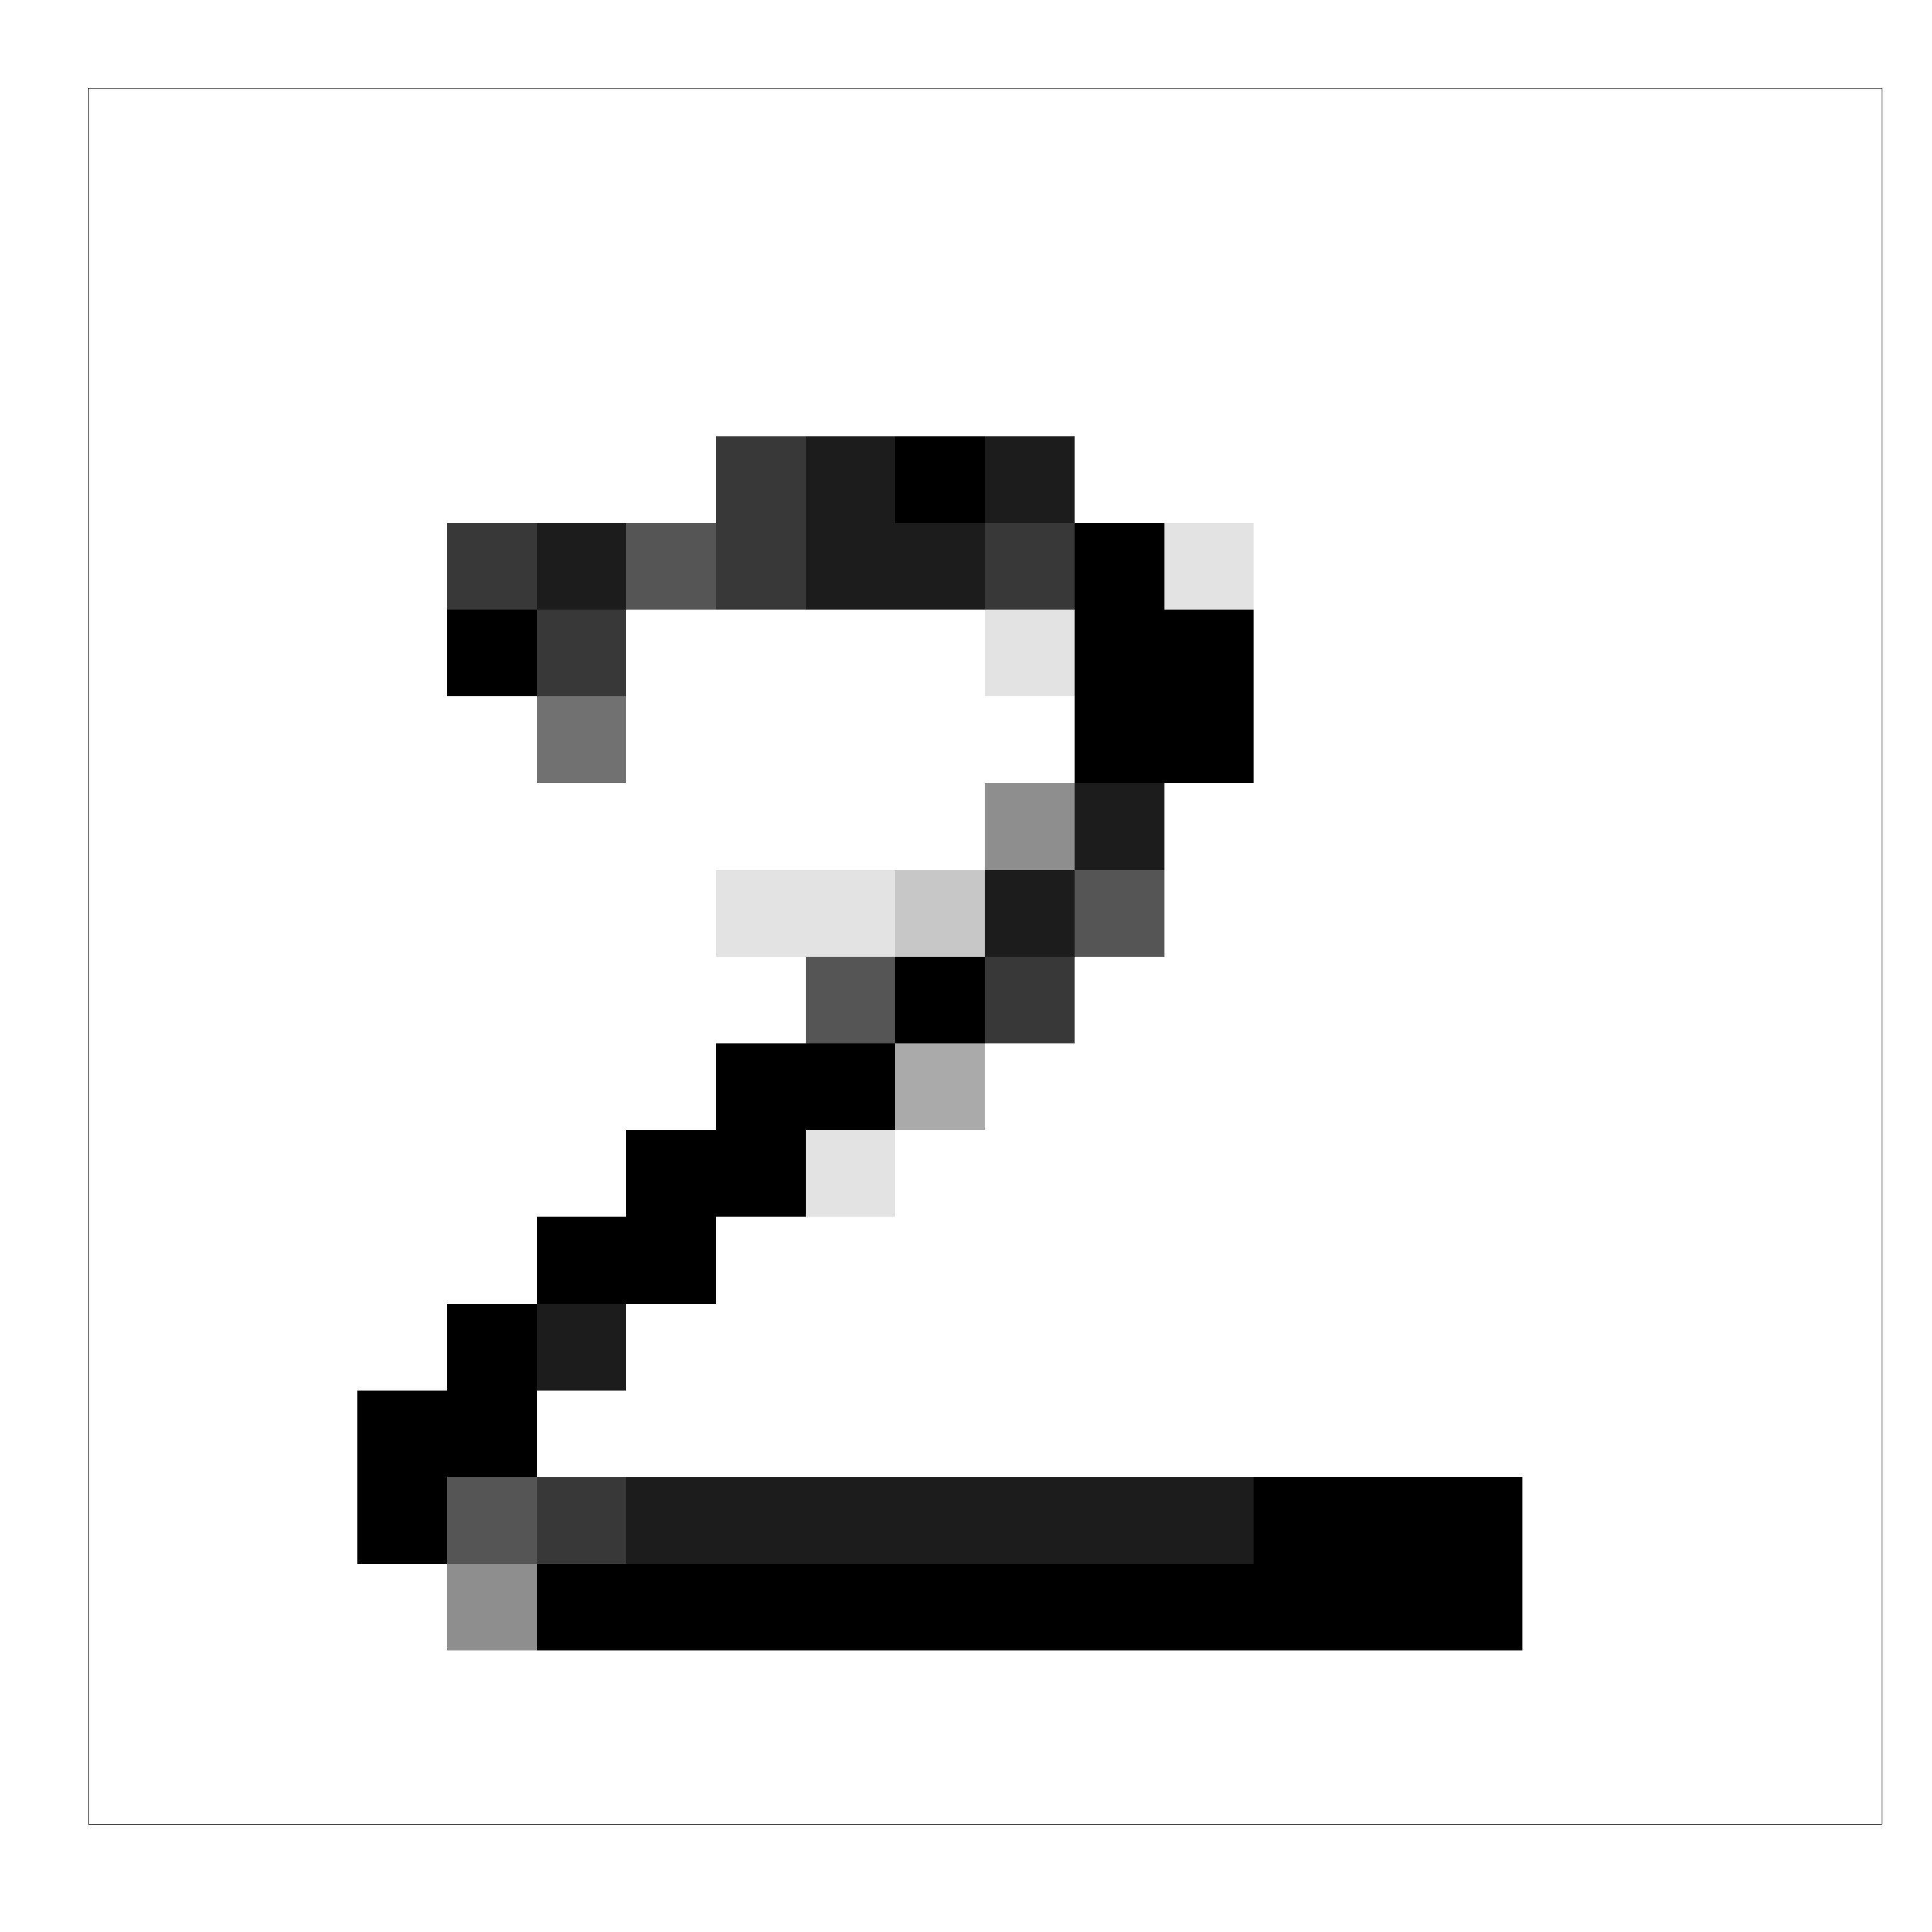
\includegraphics[width = \textwidth]{graphics/bins_10}
        \caption{10 bins.}
    \end{subfigure}
    \begin{subfigure}{0.22\textwidth}
        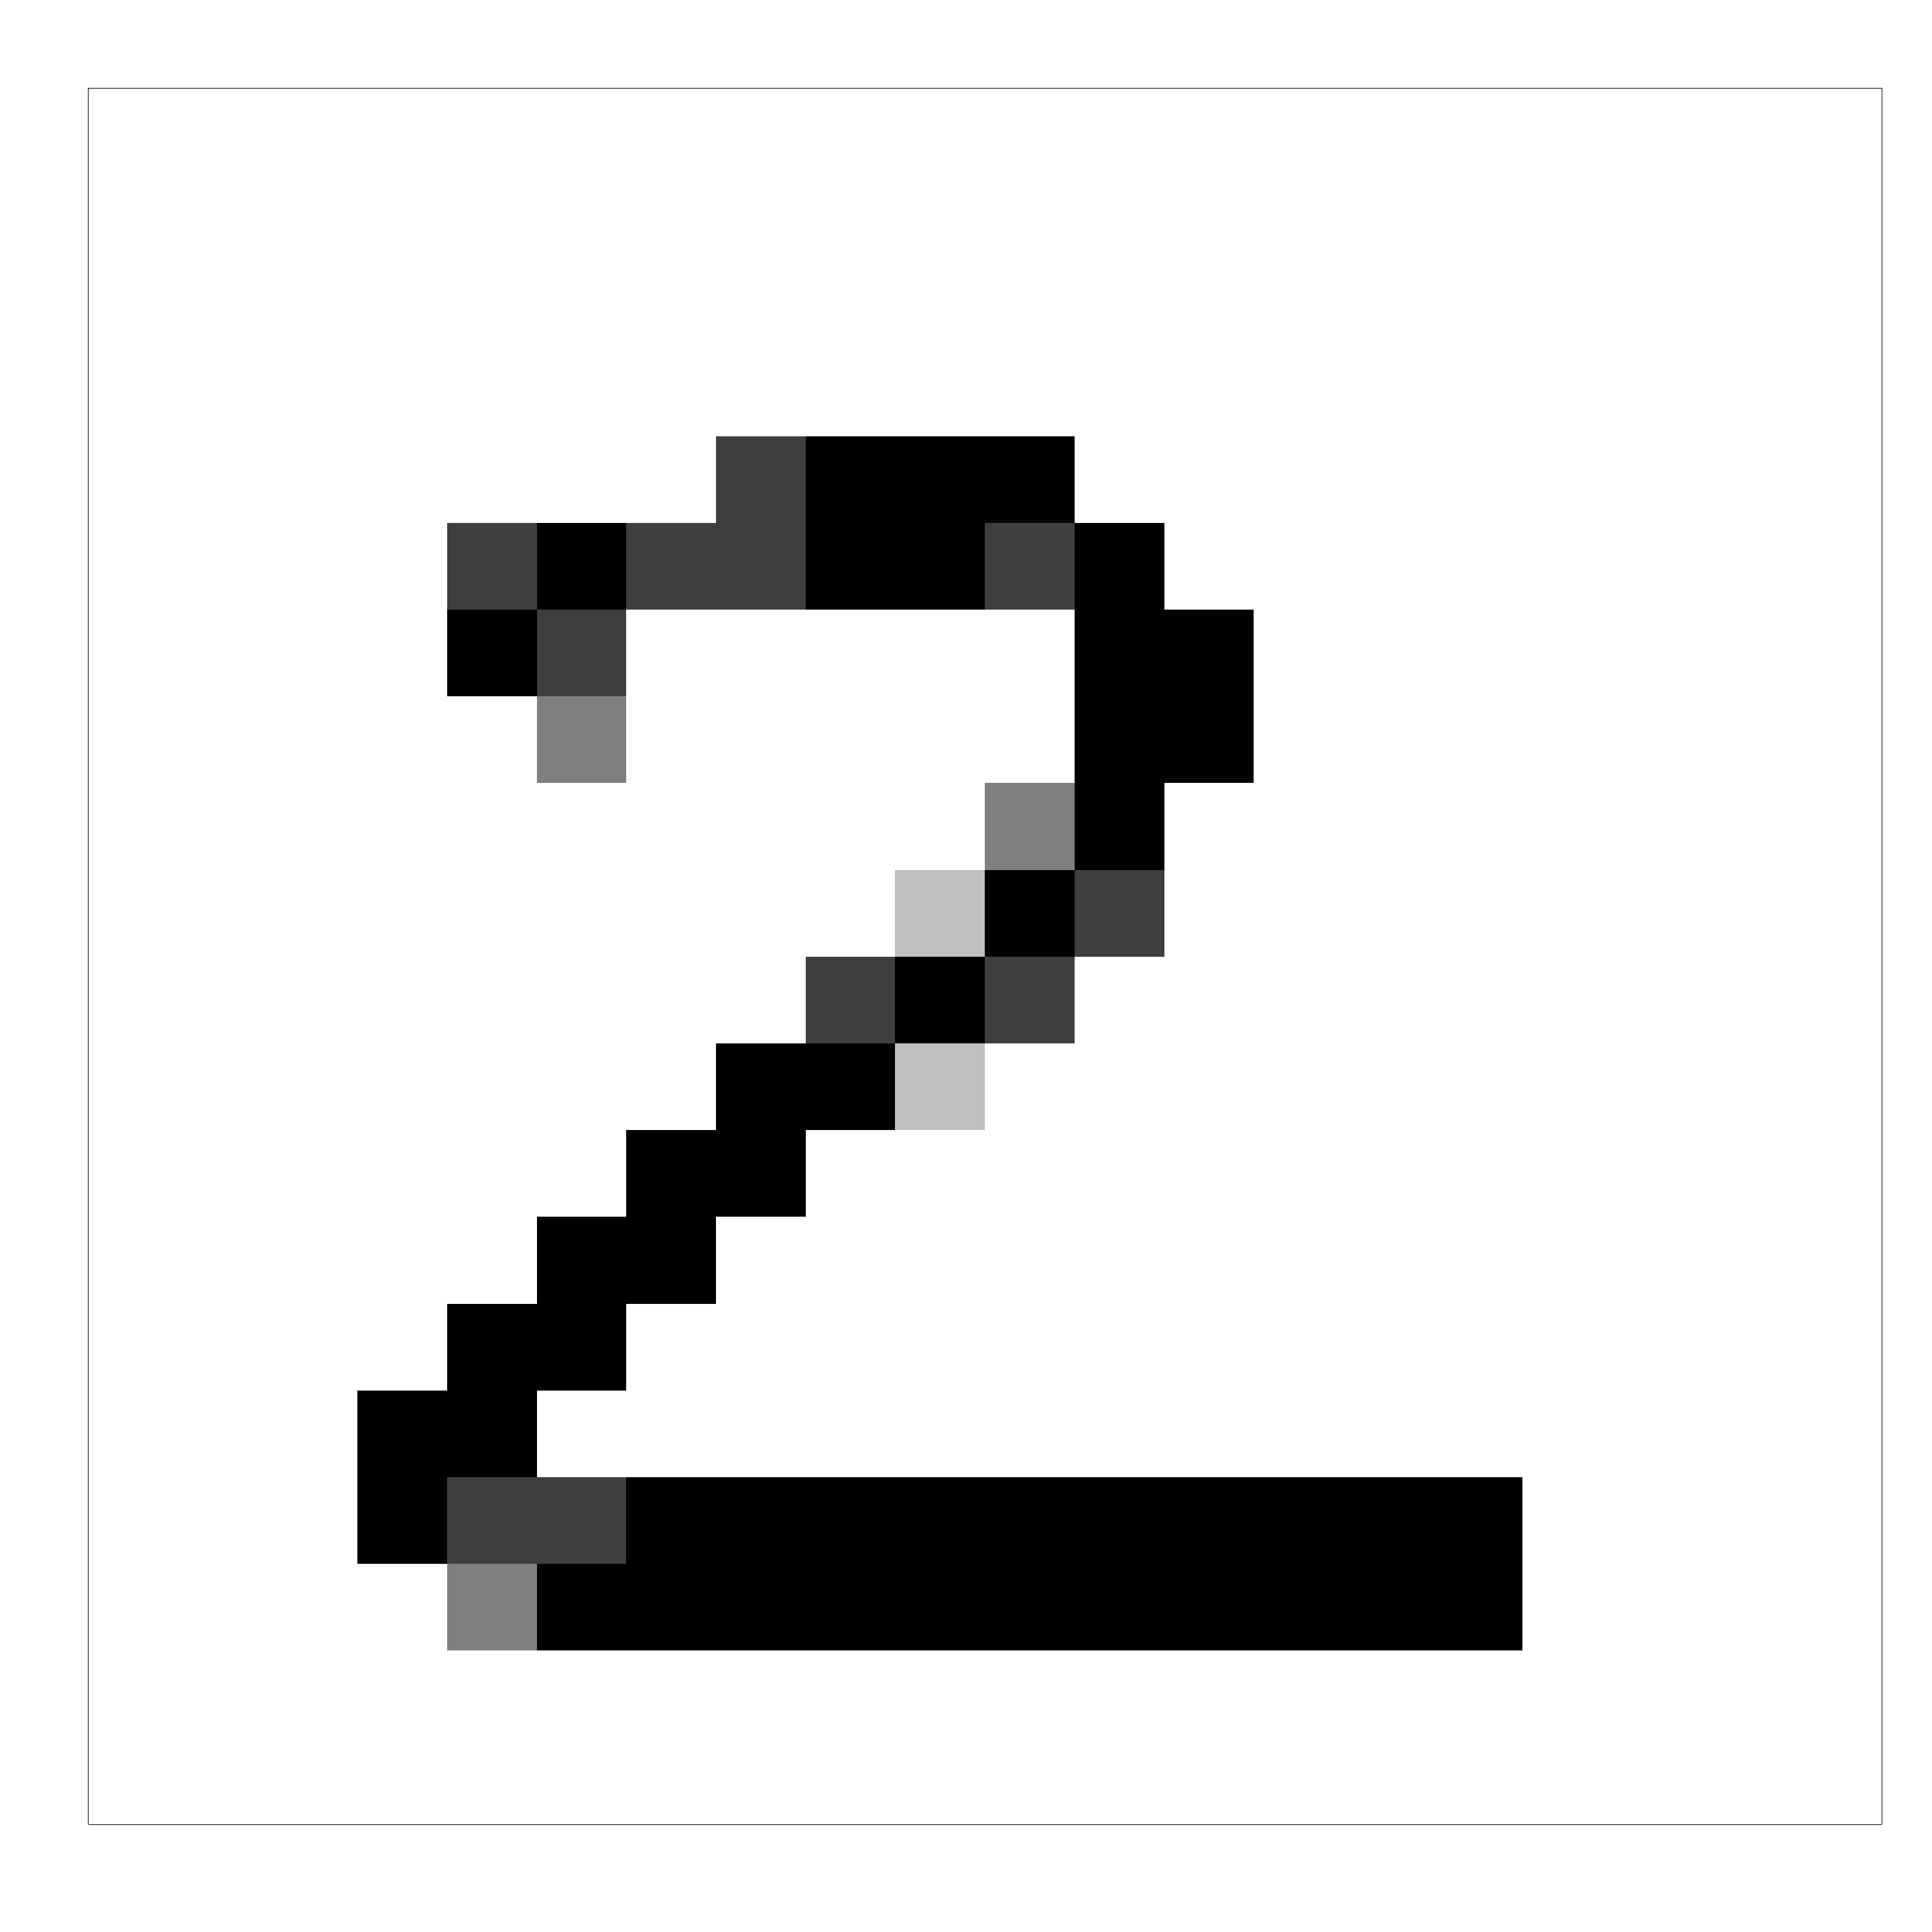
\includegraphics[width = \textwidth]{graphics/bins_5}
        \caption{5 bins.}
    \end{subfigure}
    \begin{subfigure}{0.22\textwidth}
        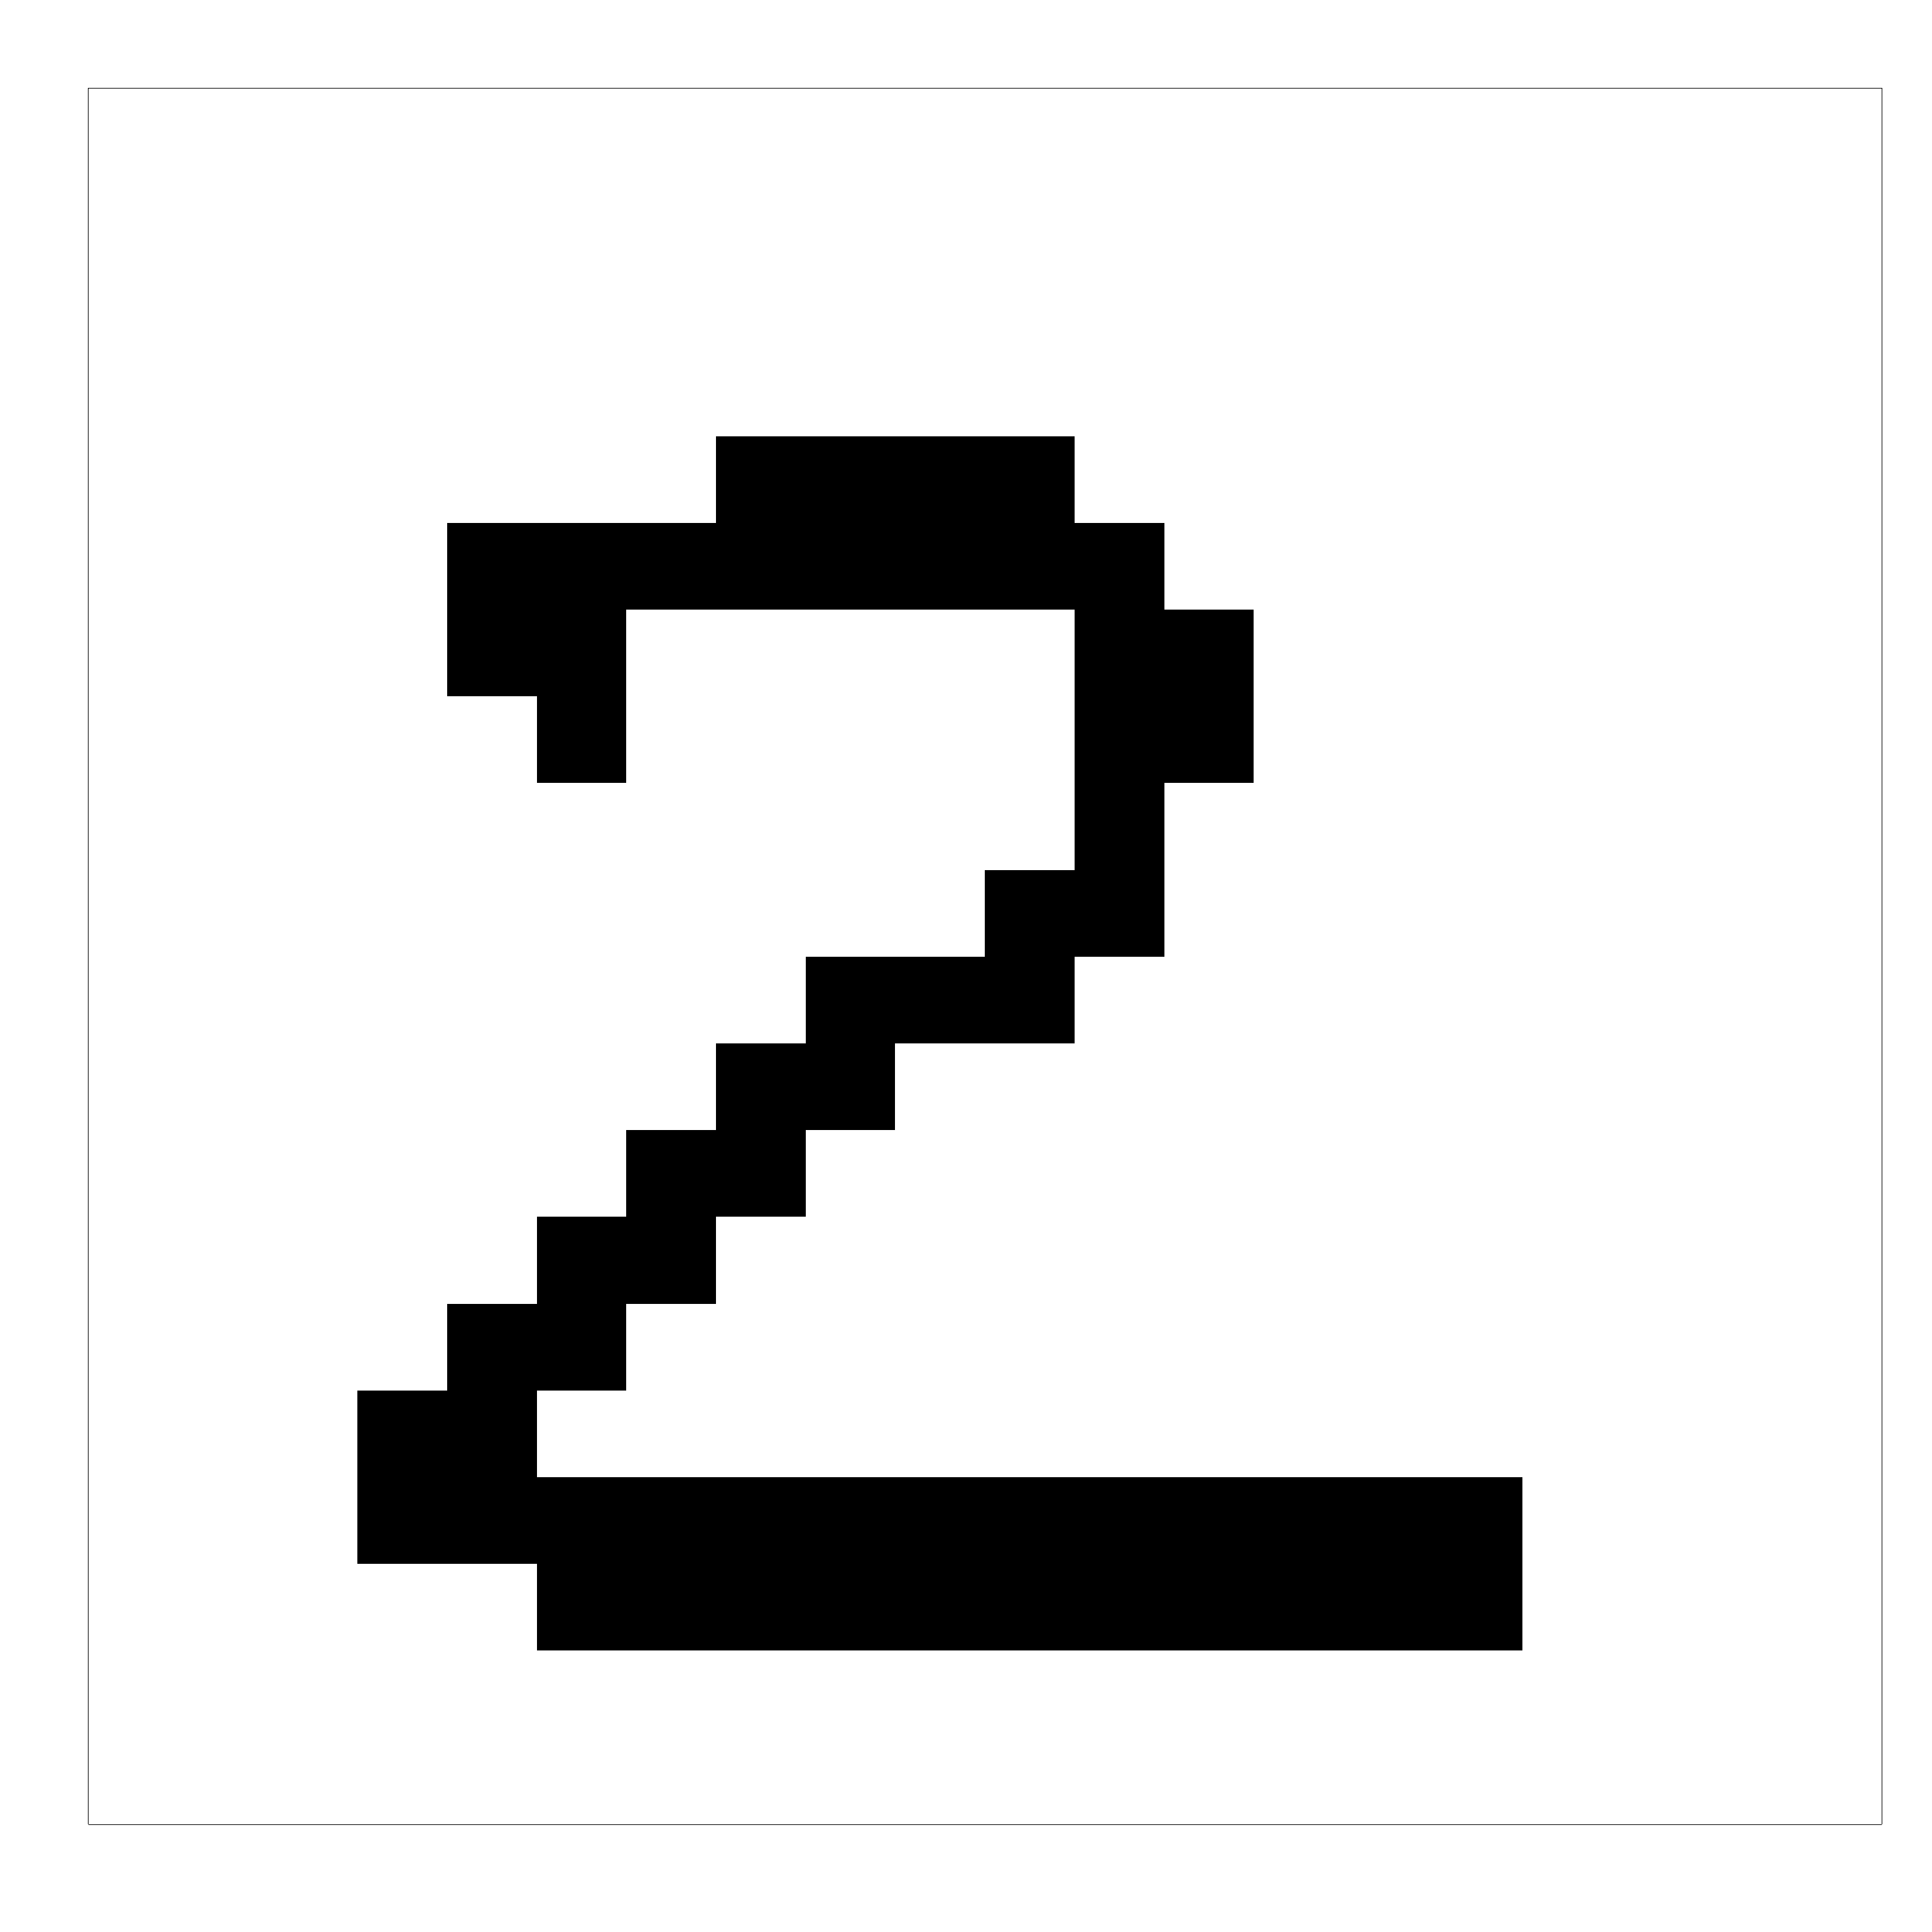
\includegraphics[width = \textwidth]{graphics/bins_2}
        \caption{2 bins.}
    \end{subfigure}
\caption{Visualization of the binning.}
\label{fig:effect_of_binning}
\end{figure}

